\documentclass[document.tex]{subfiles}
\begin{document}

\chapter {Prototypes}
\label {ch:prototypes}

In order to select a workflow framework for use in the project, a simple prototype application was constructed in both Ruote and Stonepath. The prototype application is designed around features that seemed like a good fit for the capabilities of workflow frameworks, rather than any real-world use case.


\sectionnote {BM}
\section {Overview of the Prototype Application}
\label {sec:overview-of-the-prototype-application}

\todo {Drop the reference, and specify what criteria we were evaluating in-line}

The prototype application was designed to encompass as many of the criteria in section \ref{sec:evaluation-questions} as possible in a small demonstration application. A somewhat contrived issue tracking system was designed to match these criteria.

The issue tracking system has three classes of users: reporters, developers, and project managers. Reporters are users who are responsible for reporting bugs, and providing information more information on request. Developers claim bugs from the pool of open issues, implement a fix, and then sign off on the issue. Project managers consult with developers and reporters, and assign a deployment date for the fix. All classes of users can view and comment on bugs, though they are restricted to perform only the following actions:
\begin{itemize}
\item reporters may only create issues;
\item developers may only claim issues that have not yet been claimed, and can only sign off on issues that they have claimed; and
\item project managers may only set the deployment date on issues.
\end{itemize}

Once a developer has signed off on an issue, and a project manager has set a deployment date, the issue is closed. Developers and project managers may sign off and set deployment dates in any order - though this is a somewhat unrealistic requirement, it is a good example of a pair of parallel activities. Finally, if a developer holds an issue for a week with, then the issue reverts to an unclaimed state.


\sectionnote {BM}
\section {Stonepath Prototyping Results}
\label {sec:stonepath-prototyping-results}

The requirements for the issue tracking system were translated into the state machine in Figure \ref{fig:stonepath-prototype-state-machine}. The state machine corresponds to the state of an issue - each action taken by a developer or product manager on an issue has an equivalent event. A developer claiming an issue generates a \verb!claim! event, while a developer signing off on an issue or a project manager setting the deployment date generates a \verb!close! event. As both a sign off and a deployment date are necessary for an issue to be closed, the closed state is guarded by the \verb!completed?! method.

\begin{figure}[!ht]
\centering \includegraphics[height=5in]{./img/prototypes/stonepath-state-machine}
\caption{State chart for issues in the prototype issue tracking system described in section \ref{sec:overview-of-the-prototype-application}}
\label{fig:stonepath-prototype-state-machine}
\end{figure}

The state machine model also includes a \verb!timeout! event which is triggered seven days after the in progress state is entered. The timeout was omitted from the prototype to save time, as it was not considered a risk -- several libraries already exist for Rails that provide delayed execution of method calls, as is discussed further in section \ref{sec:4ys-handling-deadlines}.

Additionally, the model also includes actions to create and destroy tasks when appropriate. Though this appeared to the be correct way to model participation in a workflow when the state machine was designed, it was discarded in the implementation, as described below.

The state machine was translated to a Ruby on Rails application, which is available at \url{https://github.com/WorkflowsOnRails/stonepath-timeboxed-example}. The application was implemented from the bottom up. First a workitem was implemented for issues, as demonstrated in the code snippet in Figure \ref{fig:stonepath-prototype-workitem}. Next, workbenches were created for roles and users. Finally, a generic task type was defined to associate workitems and workbenches. After the model was completed, authentication was implemented using Devise (described in more detail in section \ref{sec:4ys-authentication}) , and the model was wrapped with appropriate views and controllers to drive the application.

\begin{figure}[!ht]
  \begin{lstlisting}
class Issue < ActiveRecord::Base
  include StonePath::WorkItem
  owned_by :user  # owned by the initial reporter
  tasked_through :task
  state_machine do
    state :pending, initial: true,
      after_enter: [:create_claim_task, :create_deploy_task],
      after_exit: :destroy_claim_task
    state :in_progress, after_enter: :create_develop_task,
      after_exit: :destroy_develop_task
    state :closed, after_enter: :destroy_deploy_task

    event :claim do
      transitions from: :pending, to: :in_progress
    end

    event :timeout do
      transitions from: :in_progress, to: :pending
    end

    event :close do
      transitions from: :in_progress, to: :closed, guard: :completed?
    end
  end

  def completed?
    signed_off and deployment_date.present?
  end

  # ... other scopes, associations, validations and methods ...
end
  \end{lstlisting}
  \caption{Implementation of the state machine from Figure \ref{fig:stonepath-prototype-state-machine} as a Stonepath work item}
  \label{fig:stonepath-prototype-workitem}
\end{figure}

The entire prototype was simple to design and implement in Stonepath, requiring only an afternoon to complete. However, the prototype revealed several possible areas of improvement for Stonepath, such as:

\paragraph{Parallel activities:} Stonepath and AASM do not have the ability to represent sub-states, which makes it difficult to represent parallel activities. This forces developers to employ ad hoc solutions, such as the \verb!completed?! guard used in Figure \ref{fig:stonepath-prototype-workitem}. This guards ensures that the completion of the deployment or development activity does not advance the state of the workflow until the other activity has completed as well. This limitation makes it more difficult to modify workflows, as extending the duration of a parallel activity might require changing guards on activities that it previously ran in parallel with.

\paragraph{Pre-populated roles:} each role in the application was modelled with an instance of the \verb!Role! model. This allowed work items to be assigned to logical groups of users, but required extra work to put roles into the database. A seed migration had to be run whenever a production or test database was set up to create the roles, or else the application could not work. Instead of using this approach, the case study and proof-of-concept should look for a solution than specifies roles and responsibilities in the code itself, instead of the database.

\paragraph{Authorization:} Stonepath does not include an authorization layer, which means that controllers need to be written with explicit permission checks, ex. to determine if a user is a project manager before they set a deployment data. This approach seems difficult to maintain, and hardly self-documenting: the details of permission checks are scattered throughout the application, and may not all be updated at once. A workflow platform should provide a way to centralize access control in a self-documenting and easily-updated format.

\paragraph{Task modelling:} though the task model in Figure 1 was straightforward to design, it was unwieldy in practice. Stonepath represents each task as a Rails model with a polymorphic association to a workbench and a workitem. Unfortunately, polymorphic associations are implemented in Rails, and not at the database level, so it is difficult to request the developer assigned to an issue by querying the tasks. On the other hand, a developer column on an issue is easy to understand and query. Additionally, tasks are heavyweight - each task includes its own state machine, which went totally unused in the prototype application. Tasks seem to be best used to model sub-activities of an activity, while associations that need to be queried should be added to the work item itself.


\FloatBarrier

\sectionnote {AC}
\section {Ruote Prototyping Results}
\label {sec:ruote-prototyping-results}

The BPMN model shown in Figure \ref{fig:ruote-bpmn-diagram} describes how the issue tracking system works using process based methodologies. The workflow of a report begins when it is created and joins the unclaimed report pool. Developers are then able to claim the report and Managers are able to set the deployment date. Once both actions have been accomplished the developer is able to sign off the report which will then close. If the report has not been signed off after 7 days the report returns to the unclaimed report pool. Reporters are only able to create new reports. Developers are only able to claim unclaimed reports and sign off on the reports that they have claimed. Managers are only able to assign deployment dates to each claimed report.

After several weeks of work it became apparent that Ruote was not designed to easily work within a web application and the prototype was abandoned. The rest of the section will cover how the application was built and the features of Ruote.

\begin{figure}[!ht]
\centering 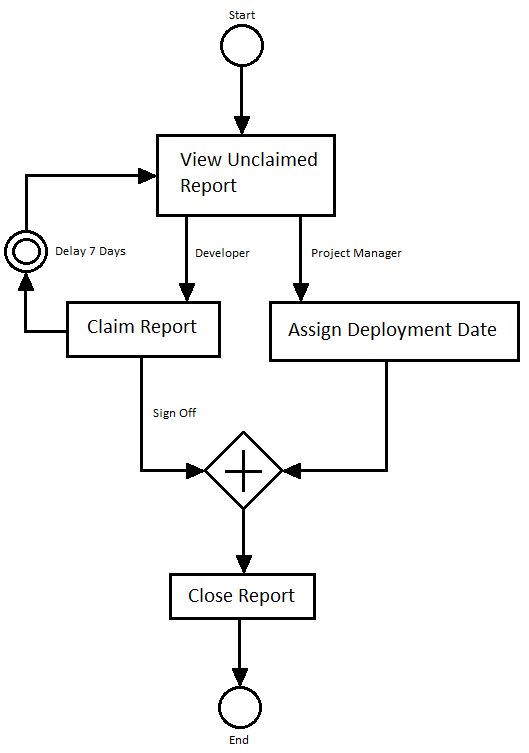
\includegraphics[height=5in]{./img/prototypes/ruote-bpmn-diagram}
\caption{BPMN for the Ruote prototype issue tracking system.}
\label{fig:ruote-bpmn-diagram}
\end{figure}

In order to integrate Ruote with rails we decided to use Ruote-Kit. Setting up a Ruote project from scratch or integrating Ruote with an existing project is simple and only involves running a script provided by the developer of Ruote-Kit. It should be noted that removing Ruote-Kit once it has been installed is unadvised due to the amount of code the script modifies.

Since the work item, the issue, was required in every process of the issue tracker only one process definition was needed to model the BPMN processes. Figure \ref{fig:ruote-prototype-process-definition} displays a code snippet that is used to describe the process definition. 

\begin{figure}[!ht]
  \begin{lstlisting}

#REPORT_OBJECT is created up here and the model is saved

pdef = Ruote.process_definition do
  unclaimed_pool
  concurrent do
    claim_issue
    sign_issue
  end
  close_issue
end

RuoteKit.engine.launch(pdef, REPORT_OBJECT) #launches the process definition

  \end{lstlisting}
  \caption{Process Definition of the Ruote prototype bug tracker.}
  \label{fig:ruote-prototype-process-definition}
\end{figure}

It is very simple to model the parallel activities \verb!claim_issue! and \verb!sign_issue! by wrapping them inside a \verb!concurrent do! statement. The process definition starts at \verb!unclaimed_pool! by invoking the \verb!on_workitem! method of every participant involved in that process. Once the process definition receives replies from all involved participants it invokes the next two processes at the same time because of the \verb!concurrent do!. Before it can move on it must wait for all the replies from both the \verb!claim_issue! participants and the \verb!sign_issue! participants.

Since Ruote is based off BPMN it easily allows the concept of roles to be implemented by creating participants for each role. The code snippet shown in Figure \ref{fig:ruote-prototype-participant-register} shows how the participants can be attached to each process. For example, the \verb!UnclaimedPoolParticipant! participant is a participant of the \verb!unclaimed_pool! process.

\begin{figure}[!ht]
  \begin{lstlisting}
#Register each participant for use in a process definition
RuoteKit.engine.register do
  participant 'unclaimed_pool', UnclaimedPoolParticipant
  participant 'claim_issue', ClaimIssueParticipant
  participant 'sign_issue', SignIssueParticipant
  participant 'close_issue', CloseIssueParticipant
end
  \end{lstlisting}
  \caption{Registering the participants with the Dashboard.}
  \label{fig:ruote-prototype-participant-register}
\end{figure}

An example participant code snippet is shown in Figure \ref{fig:ruote-prototype-participant-code}. It should be noted that there is only a single \verb!on_workitem! method which seems to indicate that a participant should only be used for a single process. It is possible to use if statements to have a participant work for more than one process but is complex and hard to maintain. The \verb!reply! call is required in order to progress the process. If the reply call is not executed the process will wait forever or until some other condition is met.

\begin{figure}[!ht]
  \begin{lstlisting}
class UnclaimedPoolParticipant
  include Ruote::LocalParticipant

  def on_workitem
    # the report_id is passed between participants and stored
    # in the workitem
    report = Report.find(workitem.lookup(id))
    --- do work on the report here ---
    reply #call to the process to notify work has finished
  end

  def on_cancel
    #called when workitem is canceled
  end

  def on_error
    #called when an error occurs
  end
end
  \end{lstlisting}
  \caption{The framework of a participant class and its methods.}
  \label{fig:ruote-prototype-participant-code}
\end{figure}

The main problem encountered with Ruote was being unable to store data within the work item object required to pass data between processes. The process of storing information was complicated due to the fact the information comes into rails as a standard web request. The information is then sent to the Ruote process and stored in a work item as a hash map. This worked really well for integers but did not work for anything more complex such as strings. In addition, there were also issues retrieving data from outside the process definition making it difficult to display what had been done to the work item.

The abstraction of the workflow provided by Ruote is a good idea on paper, but did not seem to work in practice. The rails application ended up being completely integrated with Ruote to the extent that any modification to the Ruote processes would impact the rails application significantly. For this reason Ruote is not recommended for use with web applications.


\FloatBarrier

\sectionnote {BM}
\section {Results and Discussion}

\todo {Harmonize this section with Alex's new Ruote discussion above}

After completing both prototypes, it was clear that Stonepath more appropriate for use in Rails applications than Ruote. In contrast to the Stonepath prototype (which was implemented in an afternoon), the prototype implementation using Ruote remained incomplete and was canceled after several weeks of effort.

The key problem is that Ruote's model of a workflow does not map naturally to a web application. In contrast to web servers, which operate by responding to HTTP requests with HTTP responses, Ruote models each activity in a workflow as a continuously-executing process. Developers must define the \verb!on_workitem! method of each Participant to create appropriate model instances in the database to represent the activity, carry out the activity as a sequence of request / response cycles in Rails, and then call back to Ruote using the \verb!reply! method when the activity completes. This disjointed approach is significantly more complex than the one employed by Stonepath, which defines persistent state machines on the models themselves, and allows them to respond to events generated by Rails controllers.

In fact, the only advantage offered by Ruote is the ability to define parallel workflows. However, this advantage pales against the difficulty of integrating Ruote with Rails and using it productively. Therefore, Stonepath was selected as the workflow framework to be applied in the following case study.


\end{document}
